%% bare_conf_compsoc.tex
%% V1.4b
%% 2015/08/26
%% by Michael Shell
%% See:
%% http://www.michaelshell.org/
%% for current contact information.
%%
%% This is a skeleton file demonstrating the use of IEEEtran.cls
%% (requires IEEEtran.cls version 1.8b or later) with an IEEE Computer
%% Society conference paper.
%%
%% Support sites:
%% http://www.michaelshell.org/tex/ieeetran/
%% http://www.ctan.org/pkg/ieeetran
%% and
%% http://www.ieee.org/

%%*************************************************************************
%% Legal Notice:
%% This code is offered as-is without any warranty either expressed or
%% implied; without even the implied warranty of MERCHANTABILITY or
%% FITNESS FOR A PARTICULAR PURPOSE! 
%% User assumes all risk.
%% In no event shall the IEEE or any contributor to this code be liable for
%% any damages or losses, including, but not limited to, incidental,
%% consequential, or any other damages, resulting from the use or misuse
%% of any information contained here.
%%
%% All comments are the opinions of their respective authors and are not
%% necessarily endorsed by the IEEE.
%%
%% This work is distributed under the LaTeX Project Public License (LPPL)
%% ( http://www.latex-project.org/ ) version 1.3, and may be freely used,
%% distributed and modified. A copy of the LPPL, version 1.3, is included
%% in the base LaTeX documentation of all distributions of LaTeX released
%% 2003/12/01 or later.
%% Retain all contribution notices and credits.
%% ** Modified files should be clearly indicated as such, including  **
%% ** renaming them and changing author support contact information. **
%%*************************************************************************


% *** Authors should verify (and, if needed, correct) their LaTeX system  ***
% *** with the testflow diagnostic prior to trusting their LaTeX platform ***
% *** with production work. The IEEE's font choices and paper sizes can   ***
% *** trigger bugs that do not appear when using other class files.       ***                          ***
% The testflow support page is at:
% http://www.michaelshell.org/tex/testflow/



\documentclass[conference,compsoc]{IEEEtran}
% Some/most Computer Society conferences require the compsoc mode option,
% but others may want the standard conference format.
%
% If IEEEtran.cls has not been installed into the LaTeX system files,
% manually specify the path to it like:
% \documentclass[conference,compsoc]{../sty/IEEEtran}





% Some very useful LaTeX packages include:
% (uncomment the ones you want to load)


% *** MISC UTILITY PACKAGES ***
%
%\usepackage{ifpdf}
% Heiko Oberdiek's ifpdf.sty is very useful if you need conditional
% compilation based on whether the output is pdf or dvi.
% usage:
% \ifpdf
%   % pdf code
% \else
%   % dvi code
% \fi
% The latest version of ifpdf.sty can be obtained from:
% http://www.ctan.org/pkg/ifpdf
% Also, note that IEEEtran.cls V1.7 and later provides a builtin
% \ifCLASSINFOpdf conditional that works the same way.
% When switching from latex to pdflatex and vice-versa, the compiler may
% have to be run twice to clear warning/error messages.






% *** CITATION PACKAGES ***
%
\ifCLASSOPTIONcompsoc
  % IEEE Computer Society needs nocompress option
  % requires cite.sty v4.0 or later (November 2003)
  \usepackage[nocompress]{cite}
\else
  % normal IEEE
  \usepackage{cite}
\fi
% cite.sty was written by Donald Arseneau
% V1.6 and later of IEEEtran pre-defines the format of the cite.sty package
% \cite{} output to follow that of the IEEE. Loading the cite package will
% result in citation numbers being automatically sorted and properly
% "compressed/ranged". e.g., [1], [9], [2], [7], [5], [6] without using
% cite.sty will become [1], [2], [5]--[7], [9] using cite.sty. cite.sty's
% \cite will automatically add leading space, if needed. Use cite.sty's
% noadjust option (cite.sty V3.8 and later) if you want to turn this off
% such as if a citation ever needs to be enclosed in parenthesis.
% cite.sty is already installed on most LaTeX systems. Be sure and use
% version 5.0 (2009-03-20) and later if using hyperref.sty.
% The latest version can be obtained at:
% http://www.ctan.org/pkg/cite
% The documentation is contained in the cite.sty file itself.
%
% Note that some packages require special options to format as the Computer
% Society requires. In particular, Computer Society  papers do not use
% compressed citation ranges as is done in typical IEEE papers
% (e.g., [1]-[4]). Instead, they list every citation separately in order
% (e.g., [1], [2], [3], [4]). To get the latter we need to load the cite
% package with the nocompress option which is supported by cite.sty v4.0
% and later.





% *** GRAPHICS RELATED PACKAGES ***
%
\ifCLASSINFOpdf
  \usepackage[pdftex]{graphicx}
  % declare the path(s) where your graphic files are
  \graphicspath{{../images/}}
  % and their extensions so you won't have to specify these with
  % every instance of \includegraphics
  \DeclareGraphicsExtensions{.pdf,.jpeg,.png}
\else
  % or other class option (dvipsone, dvipdf, if not using dvips). graphicx
  % will default to the driver specified in the system graphics.cfg if no
  % driver is specified.
  \usepackage[dvips]{graphicx}
  % declare the path(s) where your graphic files are
  \graphicspath{{../images/}}
  % and their extensions so you won't have to specify these with
  % every instance of \includegraphics
  \DeclareGraphicsExtensions{.eps}
\fi
% graphicx was written by David Carlisle and Sebastian Rahtz. It is
% required if you want graphics, photos, etc. graphicx.sty is already
% installed on most LaTeX systems. The latest version and documentation
% can be obtained at: 
% http://www.ctan.org/pkg/graphicx
% Another good source of documentation is "Using Imported Graphics in
% LaTeX2e" by Keith Reckdahl which can be found at:
% http://www.ctan.org/pkg/epslatex
%
% latex, and pdflatex in dvi mode, support graphics in encapsulated
% postscript (.eps) format. pdflatex in pdf mode supports graphics
% in .pdf, .jpeg, .png and .mps (metapost) formats. Users should ensure
% that all non-photo figures use a vector format (.eps, .pdf, .mps) and
% not a bitmapped formats (.jpeg, .png). The IEEE frowns on bitmapped formats
% which can result in "jaggedy"/blurry rendering of lines and letters as
% well as large increases in file sizes.
%
% You can find documentation about the pdfTeX application at:
% http://www.tug.org/applications/pdftex





% *** MATH PACKAGES ***
%
%\usepackage{amsmath}
% A popular package from the American Mathematical Society that provides
% many useful and powerful commands for dealing with mathematics.
%
% Note that the amsmath package sets \interdisplaylinepenalty to 10000
% thus preventing page breaks from occurring within multiline equations. Use:
%\interdisplaylinepenalty=2500
% after loading amsmath to restore such page breaks as IEEEtran.cls normally
% does. amsmath.sty is already installed on most LaTeX systems. The latest
% version and documentation can be obtained at:
% http://www.ctan.org/pkg/amsmath





% *** SPECIALIZED LIST PACKAGES ***
%
%\usepackage{algorithmic}
% algorithmic.sty was written by Peter Williams and Rogerio Brito.
% This package provides an algorithmic environment fo describing algorithms.
% You can use the algorithmic environment in-text or within a figure
% environment to provide for a floating algorithm. Do NOT use the algorithm
% floating environment provided by algorithm.sty (by the same authors) or
% algorithm2e.sty (by Christophe Fiorio) as the IEEE does not use dedicated
% algorithm float types and packages that provide these will not provide
% correct IEEE style captions. The latest version and documentation of
% algorithmic.sty can be obtained at:
% http://www.ctan.org/pkg/algorithms
% Also of interest may be the (relatively newer and more customizable)
% algorithmicx.sty package by Szasz Janos:
% http://www.ctan.org/pkg/algorithmicx




% *** ALIGNMENT PACKAGES ***
%
%\usepackage{array}
% Frank Mittelbach's and David Carlisle's array.sty patches and improves
% the standard LaTeX2e array and tabular environments to provide better
% appearance and additional user controls. As the default LaTeX2e table
% generation code is lacking to the point of almost being broken with
% respect to the quality of the end results, all users are strongly
% advised to use an enhanced (at the very least that provided by array.sty)
% set of table tools. array.sty is already installed on most systems. The
% latest version and documentation can be obtained at:
% http://www.ctan.org/pkg/array


% IEEEtran contains the IEEEeqnarray family of commands that can be used to
% generate multiline equations as well as matrices, tables, etc., of high
% quality.




% *** SUBFIGURE PACKAGES ***
%\ifCLASSOPTIONcompsoc
%  \usepackage[caption=false,font=footnotesize,labelfont=sf,textfont=sf]{subfig}
%\else
%  \usepackage[caption=false,font=footnotesize]{subfig}
%\fi
% subfig.sty, written by Steven Douglas Cochran, is the modern replacement
% for subfigure.sty, the latter of which is no longer maintained and is
% incompatible with some LaTeX packages including fixltx2e. However,
% subfig.sty requires and automatically loads Axel Sommerfeldt's caption.sty
% which will override IEEEtran.cls' handling of captions and this will result
% in non-IEEE style figure/table captions. To prevent this problem, be sure
% and invoke subfig.sty's "caption=false" package option (available since
% subfig.sty version 1.3, 2005/06/28) as this is will preserve IEEEtran.cls
% handling of captions.
% Note that the Computer Society format requires a sans serif font rather
% than the serif font used in traditional IEEE formatting and thus the need
% to invoke different subfig.sty package options depending on whether
% compsoc mode has been enabled.
%
% The latest version and documentation of subfig.sty can be obtained at:
% http://www.ctan.org/pkg/subfig




% *** FLOAT PACKAGES ***
%
%\usepackage{fixltx2e}
% fixltx2e, the successor to the earlier fix2col.sty, was written by
% Frank Mittelbach and David Carlisle. This package corrects a few problems
% in the LaTeX2e kernel, the most notable of which is that in current
% LaTeX2e releases, the ordering of single and double column floats is not
% guaranteed to be preserved. Thus, an unpatched LaTeX2e can allow a
% single column figure to be placed prior to an earlier double column
% figure.
% Be aware that LaTeX2e kernels dated 2015 and later have fixltx2e.sty's
% corrections already built into the system in which case a warning will
% be issued if an attempt is made to load fixltx2e.sty as it is no longer
% needed.
% The latest version and documentation can be found at:
% http://www.ctan.org/pkg/fixltx2e


%\usepackage{stfloats}
% stfloats.sty was written by Sigitas Tolusis. This package gives LaTeX2e
% the ability to do double column floats at the bottom of the page as well
% as the top. (e.g., "\begin{figure*}[!b]" is not normally possible in
% LaTeX2e). It also provides a command:
%\fnbelowfloat
% to enable the placement of footnotes below bottom floats (the standard
% LaTeX2e kernel puts them above bottom floats). This is an invasive package
% which rewrites many portions of the LaTeX2e float routines. It may not work
% with other packages that modify the LaTeX2e float routines. The latest
% version and documentation can be obtained at:
% http://www.ctan.org/pkg/stfloats
% Do not use the stfloats baselinefloat ability as the IEEE does not allow
% \baselineskip to stretch. Authors submitting work to the IEEE should note
% that the IEEE rarely uses double column equations and that authors should try
% to avoid such use. Do not be tempted to use the cuted.sty or midfloat.sty
% packages (also by Sigitas Tolusis) as the IEEE does not format its papers in
% such ways.
% Do not attempt to use stfloats with fixltx2e as they are incompatible.
% Instead, use Morten Hogholm'a dblfloatfix which combines the features
% of both fixltx2e and stfloats:
%
% \usepackage{dblfloatfix}
% The latest version can be found at:
% http://www.ctan.org/pkg/dblfloatfix




% *** PDF, URL AND HYPERLINK PACKAGES ***
%
%\usepackage{url}
% url.sty was written by Donald Arseneau. It provides better support for
% handling and breaking URLs. url.sty is already installed on most LaTeX
% systems. The latest version and documentation can be obtained at:
% http://www.ctan.org/pkg/url
% Basically, \url{my_url_here}.




% *** Do not adjust lengths that control margins, column widths, etc. ***
% *** Do not use packages that alter fonts (such as pslatex).         ***
% There should be no need to do such things with IEEEtran.cls V1.6 and later.
% (Unless specifically asked to do so by the journal or conference you plan
% to submit to, of course. )


% correct bad hyphenation here
\hyphenation{op-tical net-works semi-conduc-tor}

\usepackage[brazil, english]{babel}

\begin{document}
%
% paper title
% Titles are generally capitalized except for words such as a, an, and, as,
% at, but, by, for, in, nor, of, on, or, the, to and up, which are usually
% not capitalized unless they are the first or last word of the title.
% Linebreaks \\ can be used within to get better formatting as desired.
% Do not put math or special symbols in the title.
\title{UnB\\Redes de Computadores | 2025.1\\ Projeto 1 -  Turma 01}


% author names and affiliations
% use a multiple column layout for up to three different
% affiliations
\author{\IEEEauthorblockN{Giovanni Daldegan}
\IEEEauthorblockA{232002520\\
Ciência da Computação\\
Universidade de Brasília\\
Brasília, DF}
\and

\IEEEauthorblockN{Rodrigo Rafik}
\IEEEauthorblockA{232009502\\
Ciência da Computação\\
Universidade de Brasília\\
Brasília, DF}
\and

\IEEEauthorblockN{Rute Fernandes}
\IEEEauthorblockA{232009549\\
Ciência da Computação\\
Universidade de Brasília\\
Brasília, DF}
}

% conference papers do not typically use \thanks and this command
% is locked out in conference mode. If really needed, such as for
% the acknowledgment of grants, issue a \IEEEoverridecommandlockouts
% after \documentclass

% for over three affiliations, or if they all won't fit within the width
% of the page (and note that there is less available width in this regard for
% compsoc conferences compared to traditional conferences), use this
% alternative format:
% 
%\author{\IEEEauthorblockN{Michael Shell\IEEEauthorrefmark{1},
%Homer Simpson\IEEEauthorrefmark{2},
%James Kirk\IEEEauthorrefmark{3}, 
%Montgomery Scott\IEEEauthorrefmark{3} and
%Eldon Tyrell\IEEEauthorrefmark{4}}
%\IEEEauthorblockA{\IEEEauthorrefmark{1}School of Electrical and Computer Engineering\\
%Georgia Institute of Technology,
%Atlanta, Georgia 30332--0250\\ Email: see http://www.michaelshell.org/contact.html}
%\IEEEauthorblockA{\IEEEauthorrefmark{2}Twentieth Century Fox, Springfield, USA\\
%Email: homer@thesimpsons.com}
%\IEEEauthorblockA{\IEEEauthorrefmark{3}Starfleet Academy, San Francisco, California 96678-2391\\
%Telephone: (800) 555--1212, Fax: (888) 555--1212}
%\IEEEauthorblockA{\IEEEauthorrefmark{4}Tyrell Inc., 123 Replicant Street, Los Angeles, California 90210--4321}}




% use for special paper notices
%\IEEEspecialpapernotice{(Invited Paper)}




% make the title area
\maketitle

% As a general rule, do not put math, special symbols or citations
% in the abstract

\begin{otherlanguage}{brazil}
\begin{abstract}
O presente relatório descreve o processo de desenvolvimento do ChatWeb 2.0, uma aplicação web de chat em tempo real inspirada na estética e nas funcionalidades da internet do início dos anos 2000. Realizado no âmbito da disciplina de Redes de Computadores da Universidade de Brasília, o projeto visa aprofundar a compreensão do funcionamento de aplicações em rede, com ênfase na observação prática dos protocolos de comunicação e na arquitetura cliente-servidor.
\end{abstract}

% Brazilian Portuguese keywords
\begin{IEEEkeywords}
ChatWeb 2.0, aplicações web, protocolos de rede, comunicação em tempo real
\end{IEEEkeywords}
\end{otherlanguage}

\begin{abstract}
This report describes the development process of ChatWeb 2.0, a real-time web chat application inspired by the aesthetics and functionalities of the early 2000s internet. Conducted within the scope of the Computer Networks course at the University of Brasília, the project aims to deepen understanding of network applications operation, with emphasis on practical observation of communication protocols and client-server architecture.
\end{abstract}

% English keywords
\begin{IEEEkeywords}
ChatWeb 2.0, web applications, network protocols, real-time communication
\end{IEEEkeywords}

\begin{otherlanguage}{brazil}
    




\section{Introdução}

Este projeto consiste no desenvolvimento do ChatWeb 2.0, uma aplicação web de chat em tempo real inspirada na estética e funcionalidades da internet do início dos anos 2000. Implementado como requisito da disciplina de Redes de Computadores da Universidade de Brasília, o projeto visa demonstrar na prática os conceitos fundamentais de comunicação em rede, protocolos de transporte e arquiteturas cliente-servidor.

O ChatWeb 2.0 combina tecnologias modernas (Flask-SocketIO, WebSockets, JavaScript ES6) com um design nostálgico que remete ao Windows XP e às interfaces web clássicas. A aplicação permite que múltiplos usuários se conectem simultaneamente, criem salas de chat temáticas e troquem mensagens instantaneamente, proporcionando uma experiência autêntica da web dos anos 2000.

% Add project logo/image following academic standards
\begin{figure}[!h]
\centering

\includegraphics[width=0.3\textwidth]{../media/chatweb.png}
\caption{Logotipo do projeto no estilo gráfico ``y2k''}
\label{fig:chatweb_logo}
\end{figure}

O sistema foi projetado como uma ferramenta educacional que ilustra o funcionamento de protocolos de rede modernos em um contexto prático e visual. A interface utiliza a fonte Monaspace Neon, cores características do Windows XP e elementos visuais com efeitos de sombra e relevo que remetem aos sistemas operacionais clássicos.

O projeto aborda conceitos como gerenciamento de conexões WebSocket, sincronização de estado distribuído, arquitetura orientada a eventos e análise de tráfego de rede em tempo real. Através da implementação e análise deste sistema, é possível compreender como as comunicações bidirecionais modernas funcionam e os desafios envolvidos no desenvolvimento de aplicações web em tempo real.

\section{Fundamentação Teórica}

O ChatWeb 2.0 foi desenvolvido com base no modelo de arquitetura cliente-servidor, no qual o servidor central é responsável por gerenciar conexões, autenticações e o fluxo de mensagens, enquanto os clientes interagem com o sistema por meio de uma interface gráfica. Essa organização segue o princípio clássico da comunicação em redes, conforme discutido por Kurose e Ross em Computer Networking: A Top-Down Approach$^{[10]}$, onde o servidor centraliza a lógica da aplicação e os clientes atuam como consumidores do serviço.

Dessa forma, a aplicação foi estruturada em duas partes principais para o desenvolvimento: front-end e back-end.

O front-end do ChatWeb 2.0 foi construído inteiramente com HTML, CSS e JavaScript, adotando um design visual inspirado na estética da internet do início dos anos 2000. A interface oferece três telas principais para a interação do usuário: uma tela de login; uma tela com a lista de salas de chat disponíveis, que também permite a criação de novas salas; e, por fim, a tela de chat propriamente dita, onde os usuários podem enviar e receber mensagens em tempo real.

Para o back-end da aplicação, utilizamos a linguagem Python em conjunto com o framework Flask$^{[3]}$ para a construção de um servidor baseado na biblioteca Werkzeug. Além disso, foi empregada a extensão Flask-SocketIO$^{[4]}$, que implementa o protocolo Socket.IO para aplicações Flask. Essa biblioteca permite a comunicação bidirecional em tempo real entre cliente e servidor, viabilizando o envio e recebimento de mensagens instantâneas sem a necessidade de recarregamento da página. No lado do cliente, a biblioteca JavaScript Socket.IO foi utilizada para estabelecer conexões persistentes com o servidor e gerenciar os eventos de comunicação. Ela fornece uma API simples para emitir e escutar eventos personalizados, facilitando o desenvolvimento de interações em tempo real.

A identificação única de usuários e salas é feita por meio da biblioteca UUID, uma ferramenta nativa do Python utilizada para gerar identificadores únicos universais (UUIDs). Com ela, é possível garantir que cada cliente e sala de chat tenha um ID exclusivo, evitando conflitos e assegurando a integridade dos dados, mesmo em cenários com múltiplas conexões simultâneas.

Do ponto de vista da arquitetura de rede, a aplicação utiliza o protocolo WebSocket como principal meio de comunicação, permitindo conexões full-duplex contínuas sobre o TCP, o que reduz a latência e melhora a eficiência da troca de dados. Sobre ele, o Socket.IO atua como uma camada de abstração, oferecendo funcionalidades extras como reconexão automática, salas virtuais, eventos personalizados e suporte a diferentes formatos de dados. A conexão é iniciada via HTTP e, em seguida, atualizada para WebSocket, garantindo uma comunicação estável, rápida e confiável entre cliente e servidor.

\section{Experimento}

\subsection{Ambiente Experimental}

O desenvolvimento do ChatWeb 2.0 foi conduzido em um ambiente controlado que permitiu a análise detalhada dos protocolos de rede envolvidos na comunicação cliente-servidor. A configuração experimental foi estruturada para proporcionar observação prática dos conceitos teóricos estudados na disciplina.

\textbf{Infraestrutura de Desenvolvimento}:
O sistema foi implementado utilizando uma arquitetura cliente-servidor moderna, com backend em Python e frontend em JavaScript. O servidor Flask-SocketIO foi configurado para aceitar conexões na porta 5000, permitindo acesso de múltiplos dispositivos na rede local através do protocolo WebSocket.

\textbf{Ambiente de Rede}:
Os experimentos foram realizados em rede local (LAN), com o servidor executando em uma máquina Linux e clientes conectando através de navegadores web modernos. Esta configuração isolada permitiu análise detalhada do tráfego de rede sem interferências externas, facilitando a observação dos protocolos de comunicação em diferentes camadas.

\textbf{Ferramentas de Monitoramento}:
Para análise do comportamento da rede, utilizou-se o Wireshark$^{[5]}$ como ferramenta principal de captura e análise de pacotes. Esta ferramenta permitiu observação detalhada do estabelecimento de conexões WebSocket, identificação dos frames de dados trocados e análise do comportamento dos protocolos nas camadas física, enlace, rede, transporte e aplicação.

\section{Análise dos Resultados}

\subsection{Monitoramento de Pacotes}

Ao monitorar os pacotes transmitidos entre servidor e clientes durante o uso da aplicação, através do software Wireshark$^{[5]}$, próprio para a análise de tráfego de rede, foi possível destacar os pacotes gerados pela comunicação entre os dispositivos.

A ferramenta permitiu a inspeção das requisições HTTP dos arquivos presentes no servidor (elementos HTML, imagens, códigos em JavaScript, arquivos CSS) realizadas por parte dos clientes, além das mensagens de comunicação do SocketIO entre cliente e servidor. O tráfego desses dados permitiu que os clientes fizessem uso pleno dos recursos da aplicação: registrassem-se com nome, criassem salas de bate-papo e trocassem mensagens por elas.

No experimento conduzido, o laptop que se comunicou com o servidor será chamado de Cliente 1 e o celular, Cliente 2. A seção seguinte destrincha os resultados obtidos.

\subsection{Análise dos Resultados Obtidos}


\begin{figure}[!h]
\centering
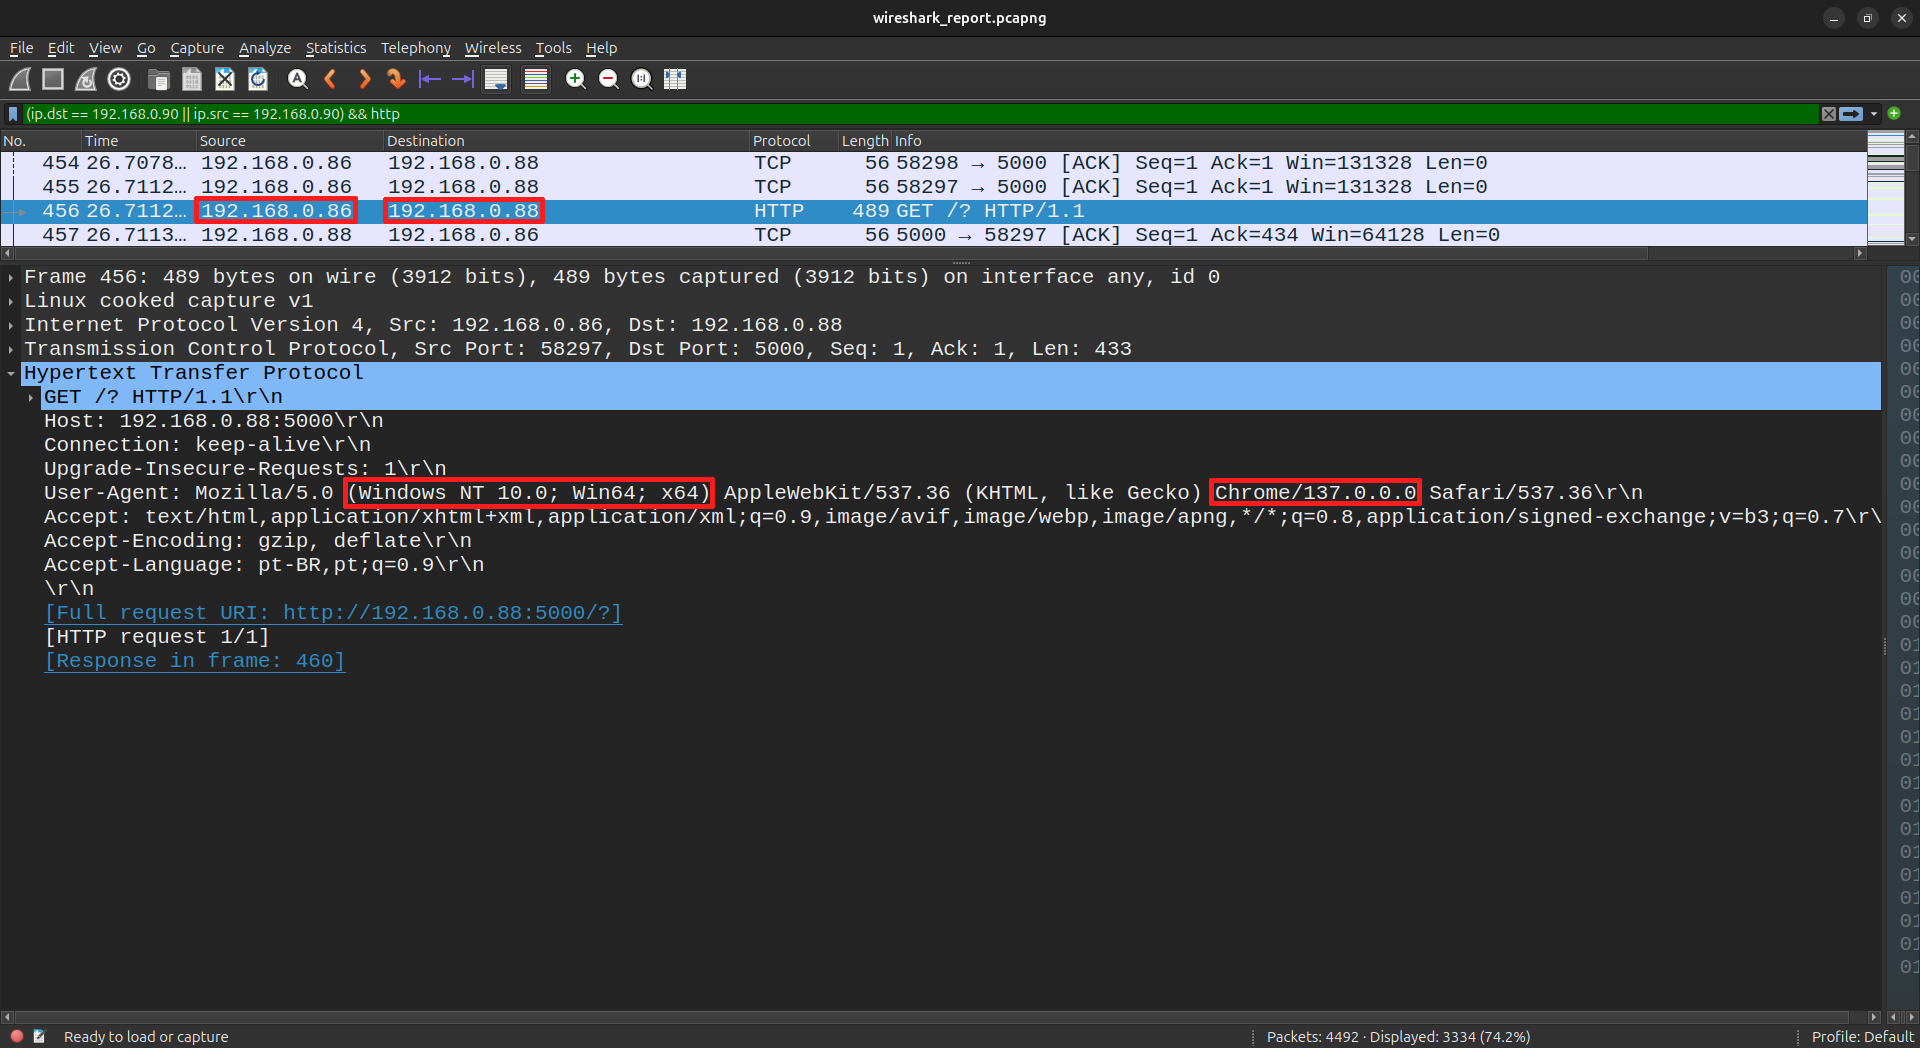
\includegraphics[width=\columnwidth]{../media/00-client0_app.png}
\caption{Requisição HTTP do índice do serviço pelo Cliente 1}
\label{fig:client1_request}
\end{figure}

\begin{figure}[!h]
\centering
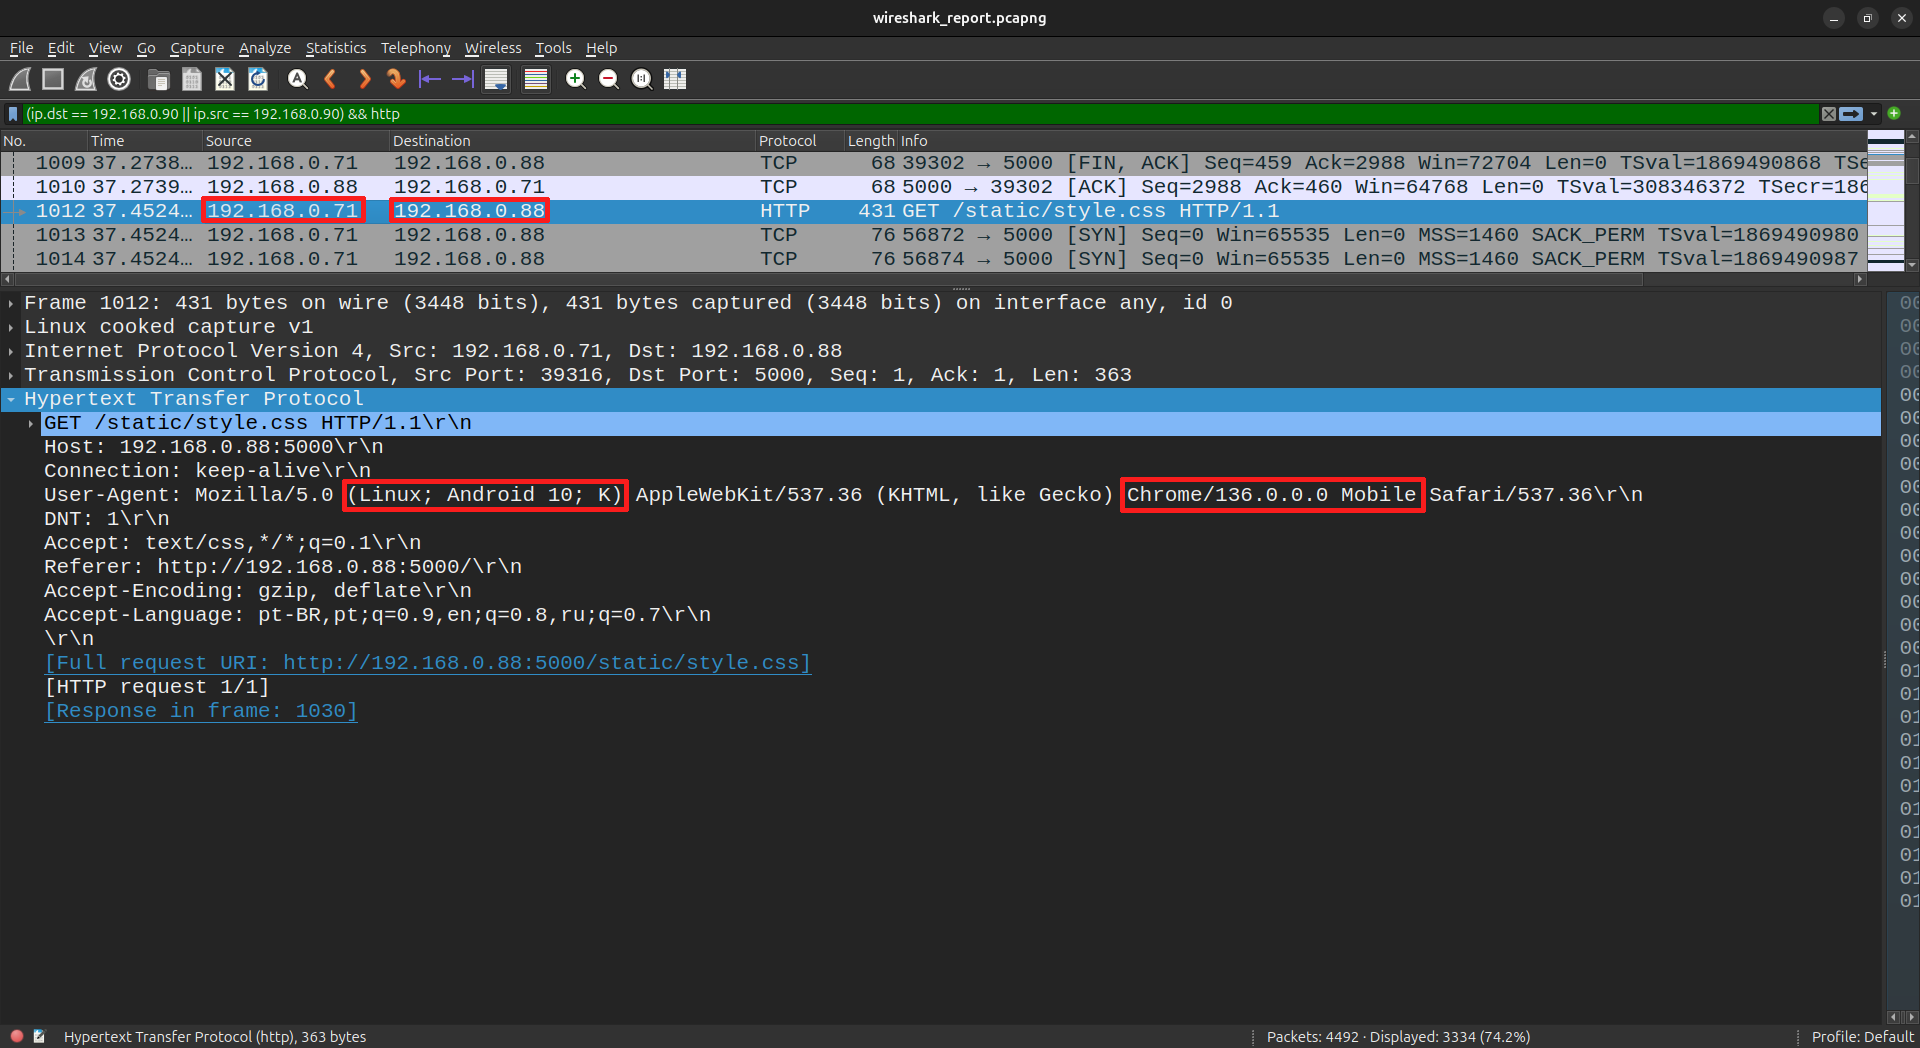
\includegraphics[width=\columnwidth]{../media/01-client1_app.png}
\caption{Requisição HTTP do índice pelo Cliente 2}
\label{fig:client2_request}
\end{figure}

\begin{figure}[!h]
\centering
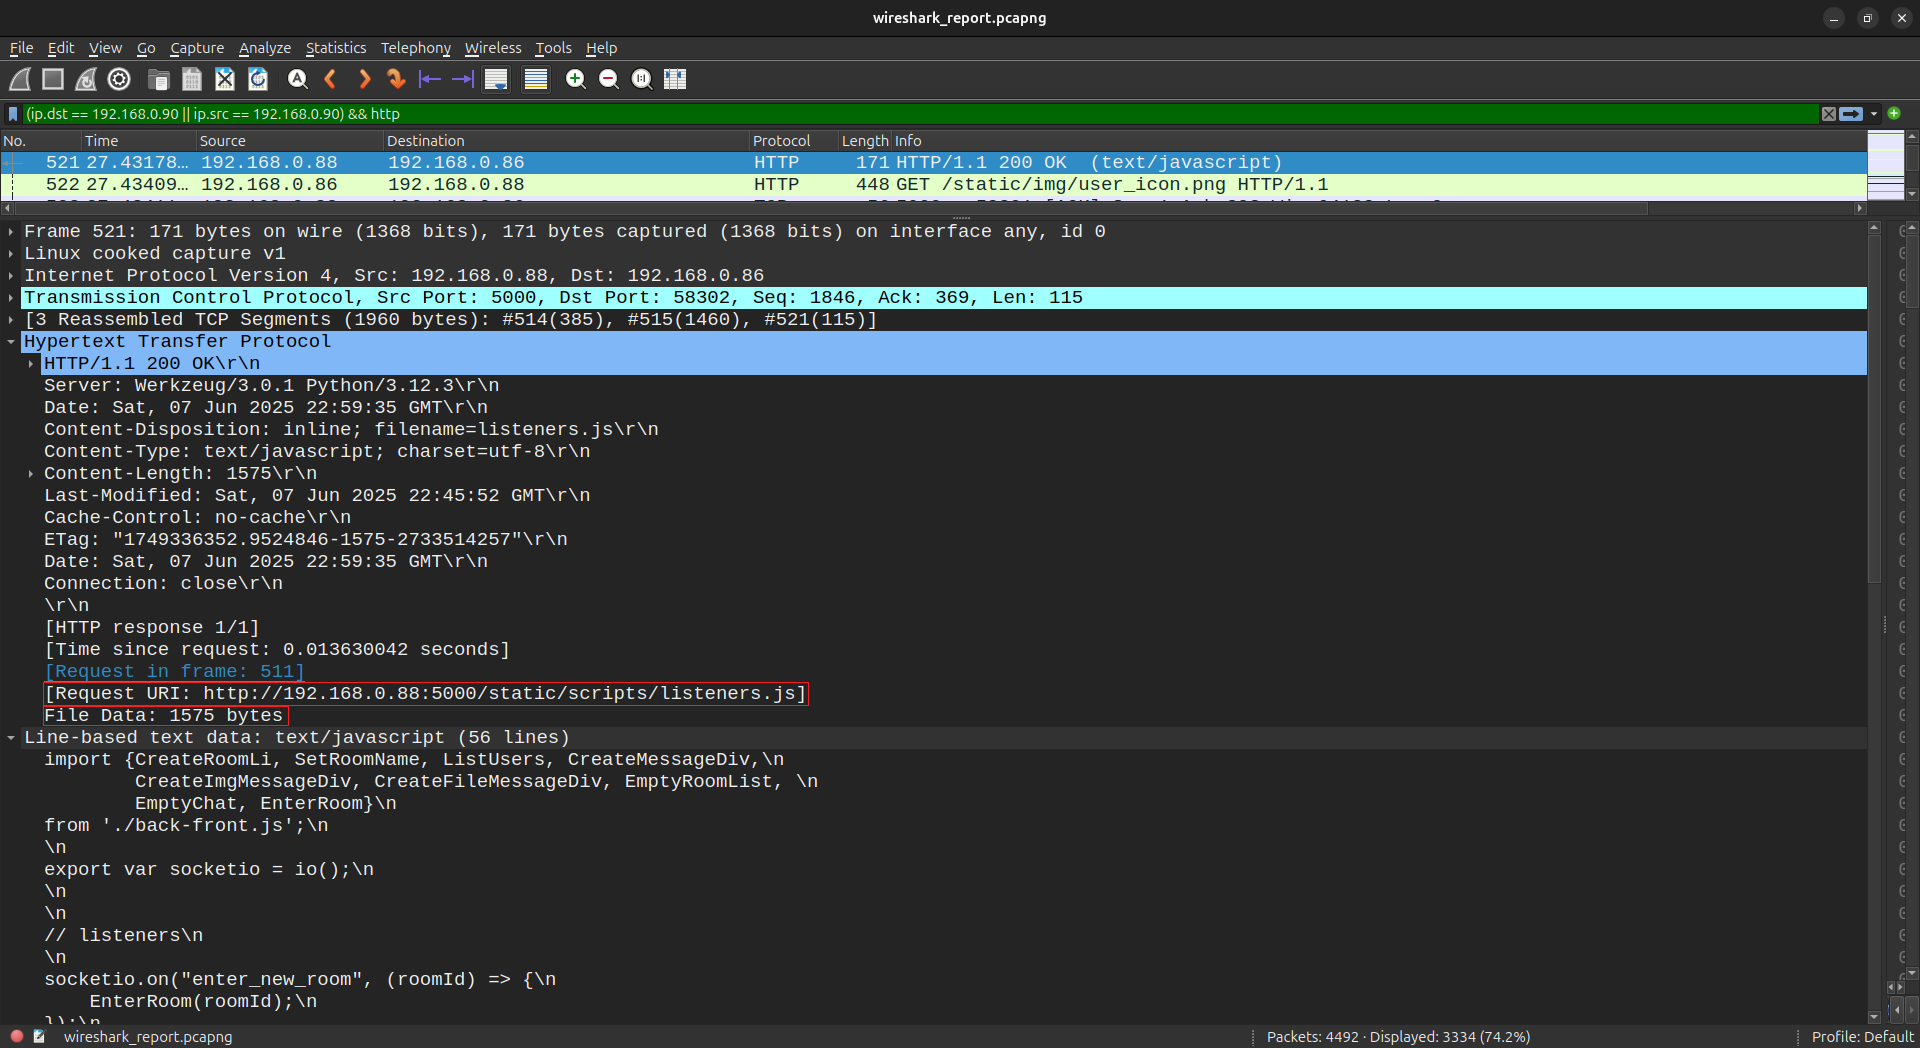
\includegraphics[width=\columnwidth]{../media/02-OK_listeners.js_file_data.png}
\caption{Resposta HTTP do servidor à requisição do arquivo ``listeners.js'' pelo Cliente 1}
\label{fig:listeners_response}
\end{figure}

\begin{figure}[!h]
\centering
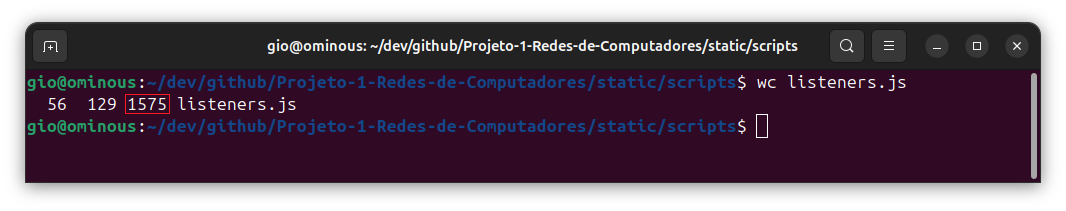
\includegraphics[width=\columnwidth]{../media/03-listeners_total_bytes.png}
\caption{Tamanho em bytes do arquivo listeners.js, obtido pelo comando ``wc''}
\label{fig:listeners_size}
\end{figure}

\begin{figure}[!h]
\centering
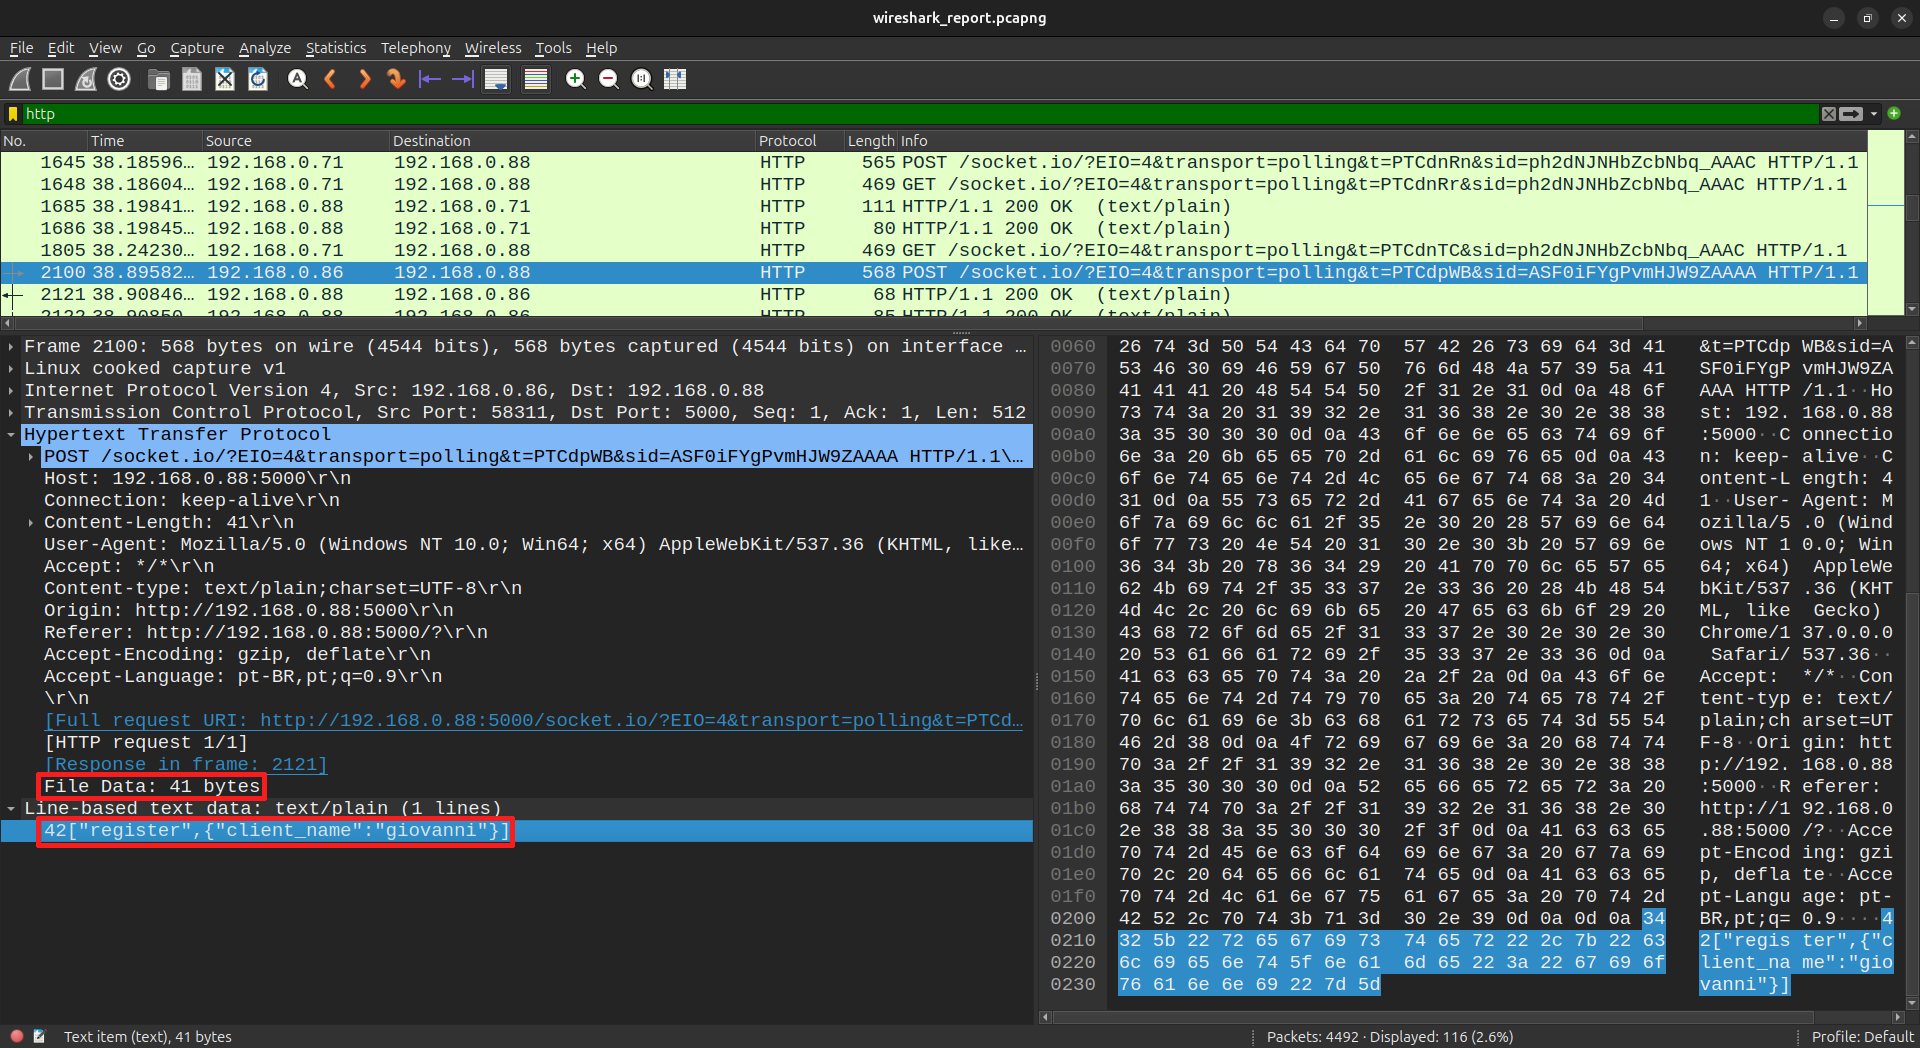
\includegraphics[width=\columnwidth]{../media/04-register.png}
\caption{Mensagem gerada pelo SocketIO presente na aplicação do Cliente 1, registrando-o com o nome ``giovanni''}
\label{fig:socketio_register}
\end{figure}

\begin{figure}[!h]
\centering
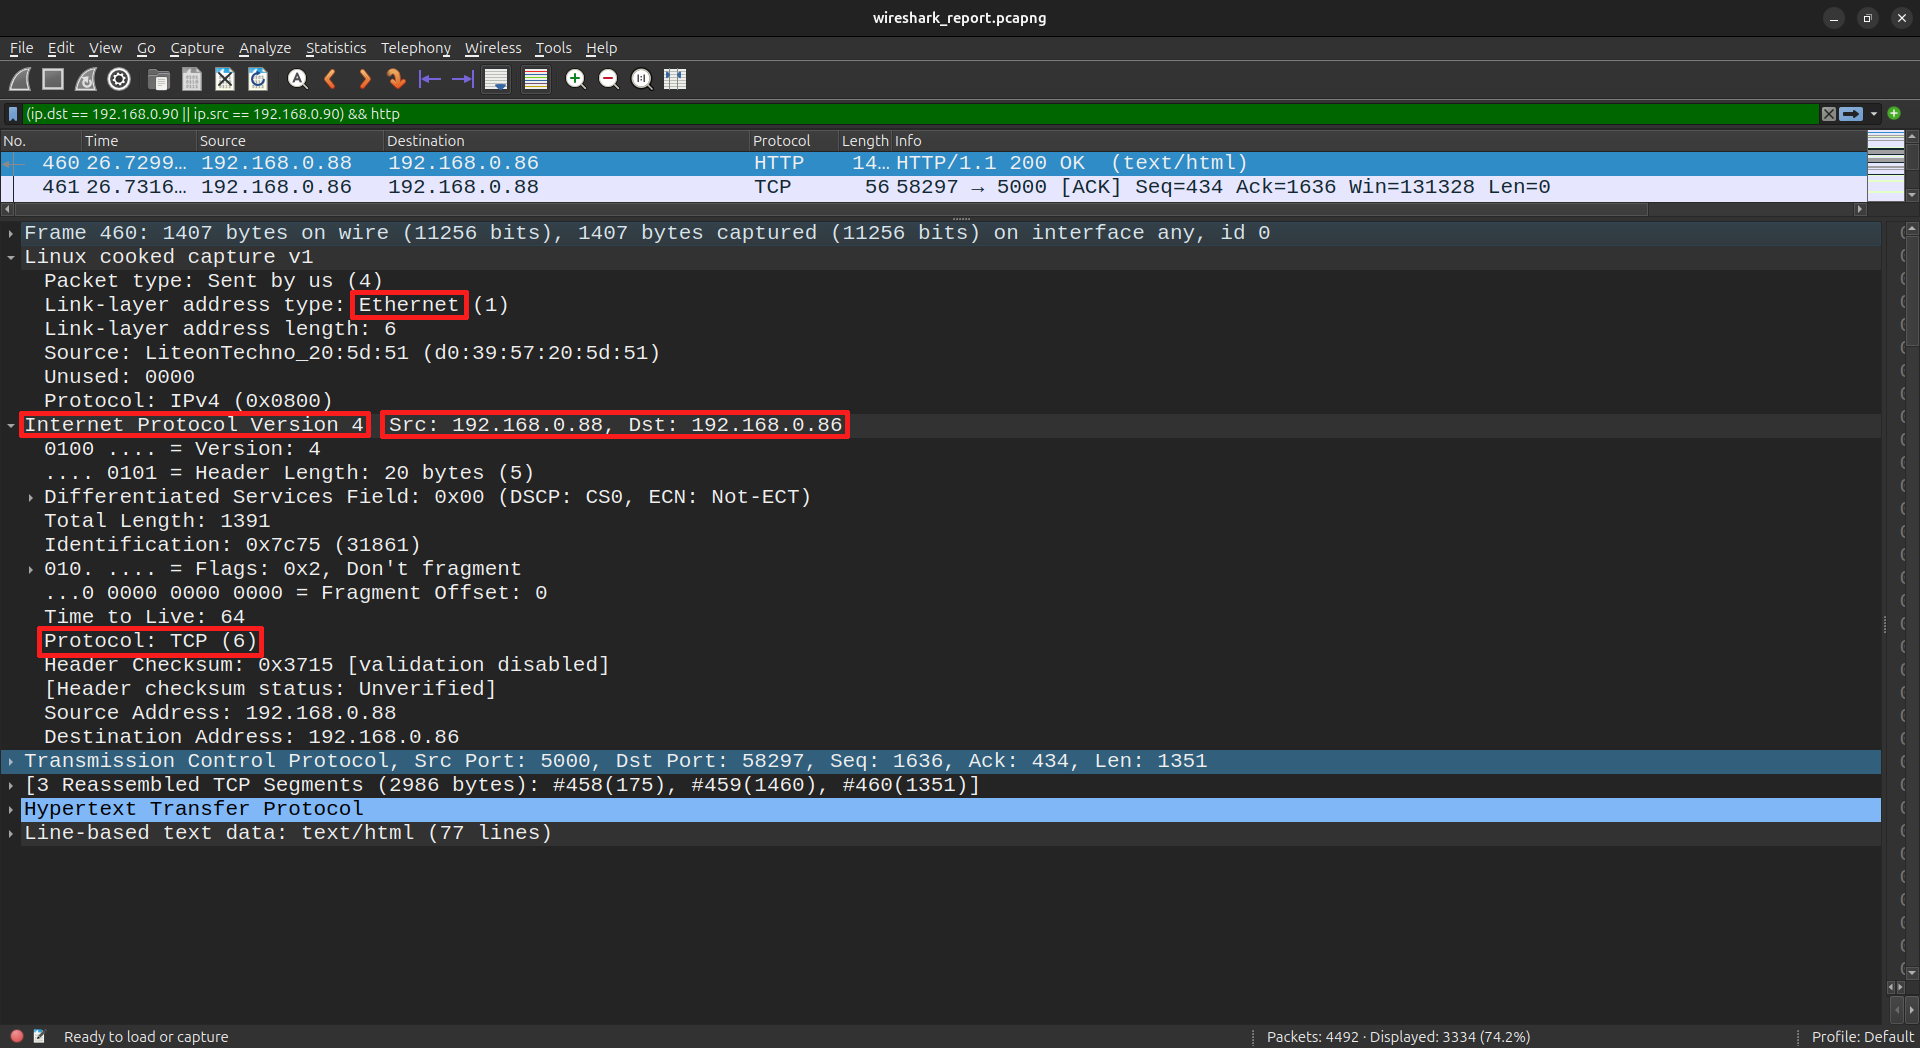
\includegraphics[width=\columnwidth]{../media/05-server_link_network.png}
\caption{Cabeçalhos de enlace e rede da resposta à primeira requisição do Cliente 1}
\label{fig:link_network_headers}
\end{figure}

\begin{figure}[!h]
\centering
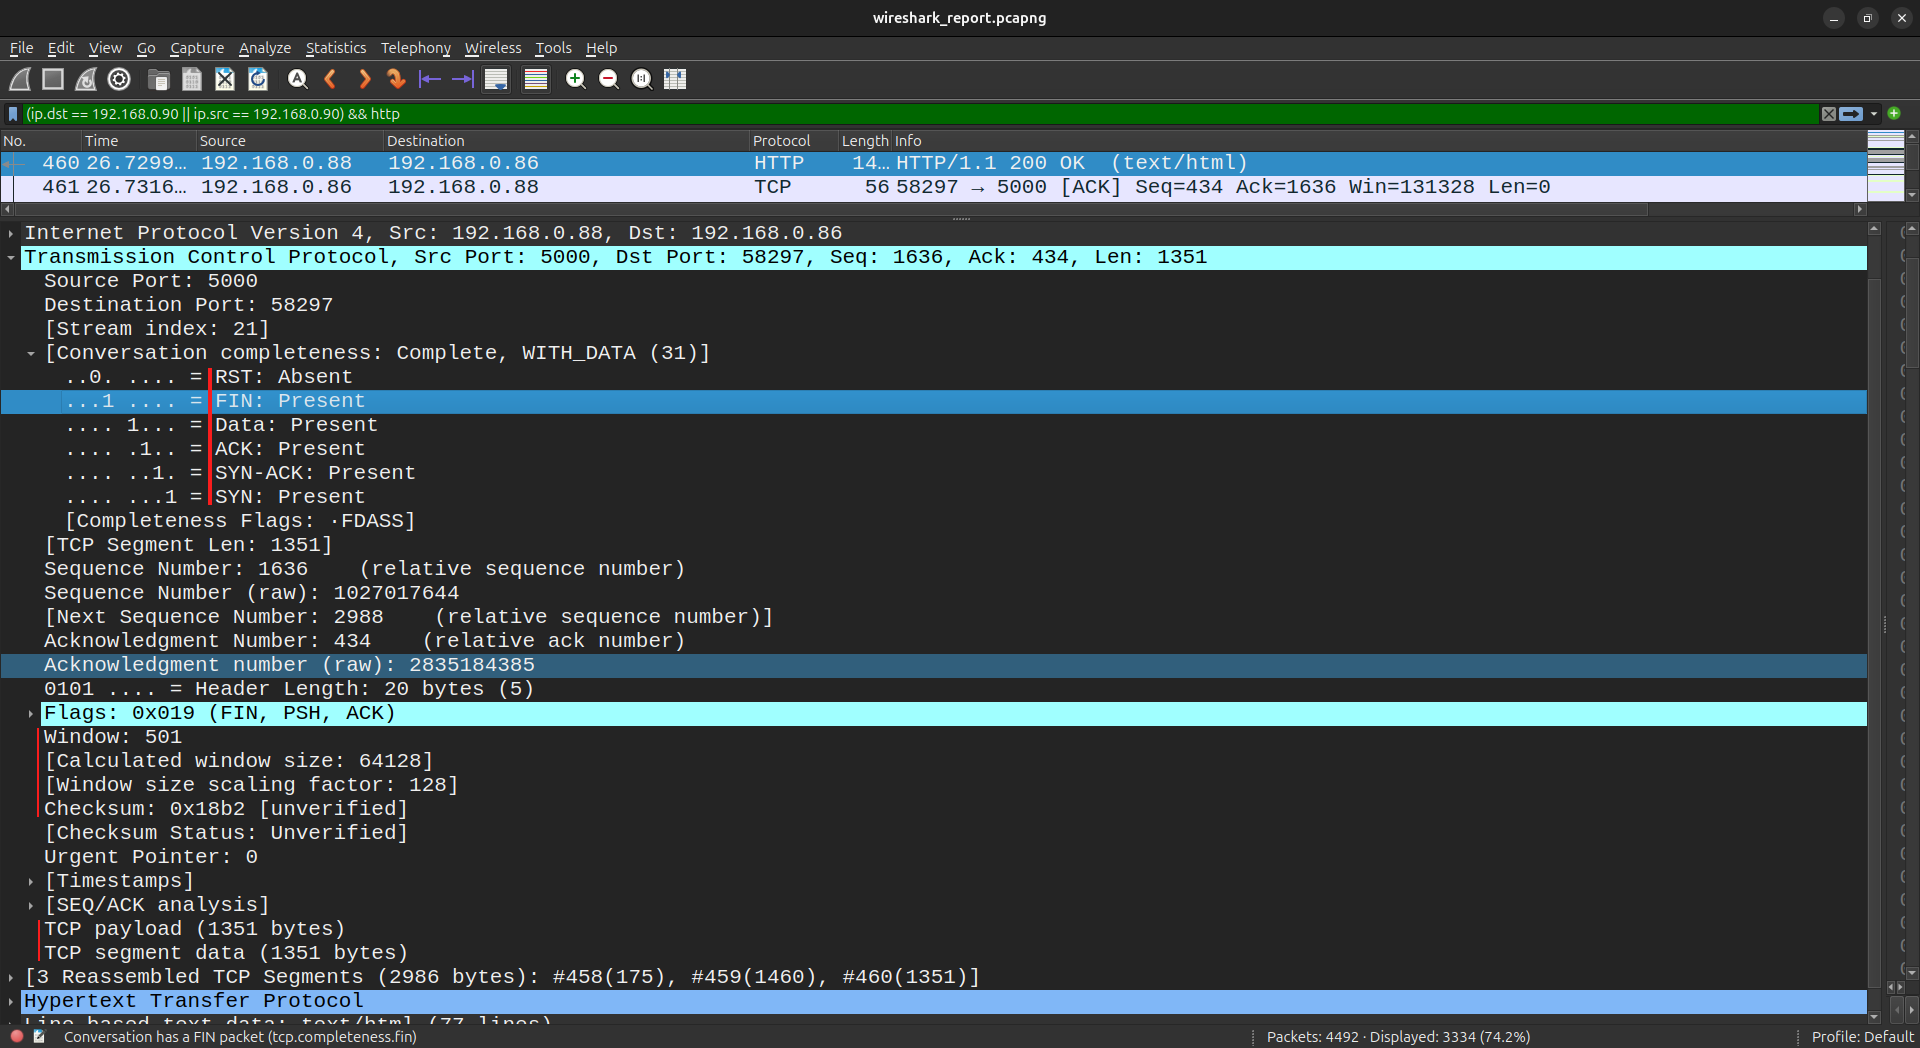
\includegraphics[width=\columnwidth]{../media/06-server_transport.png}
\caption{Cabeçalho de transporte da resposta à primeira requisição do Cliente 1}
\label{fig:transport_header}
\end{figure}

\begin{figure}[!h]
\centering
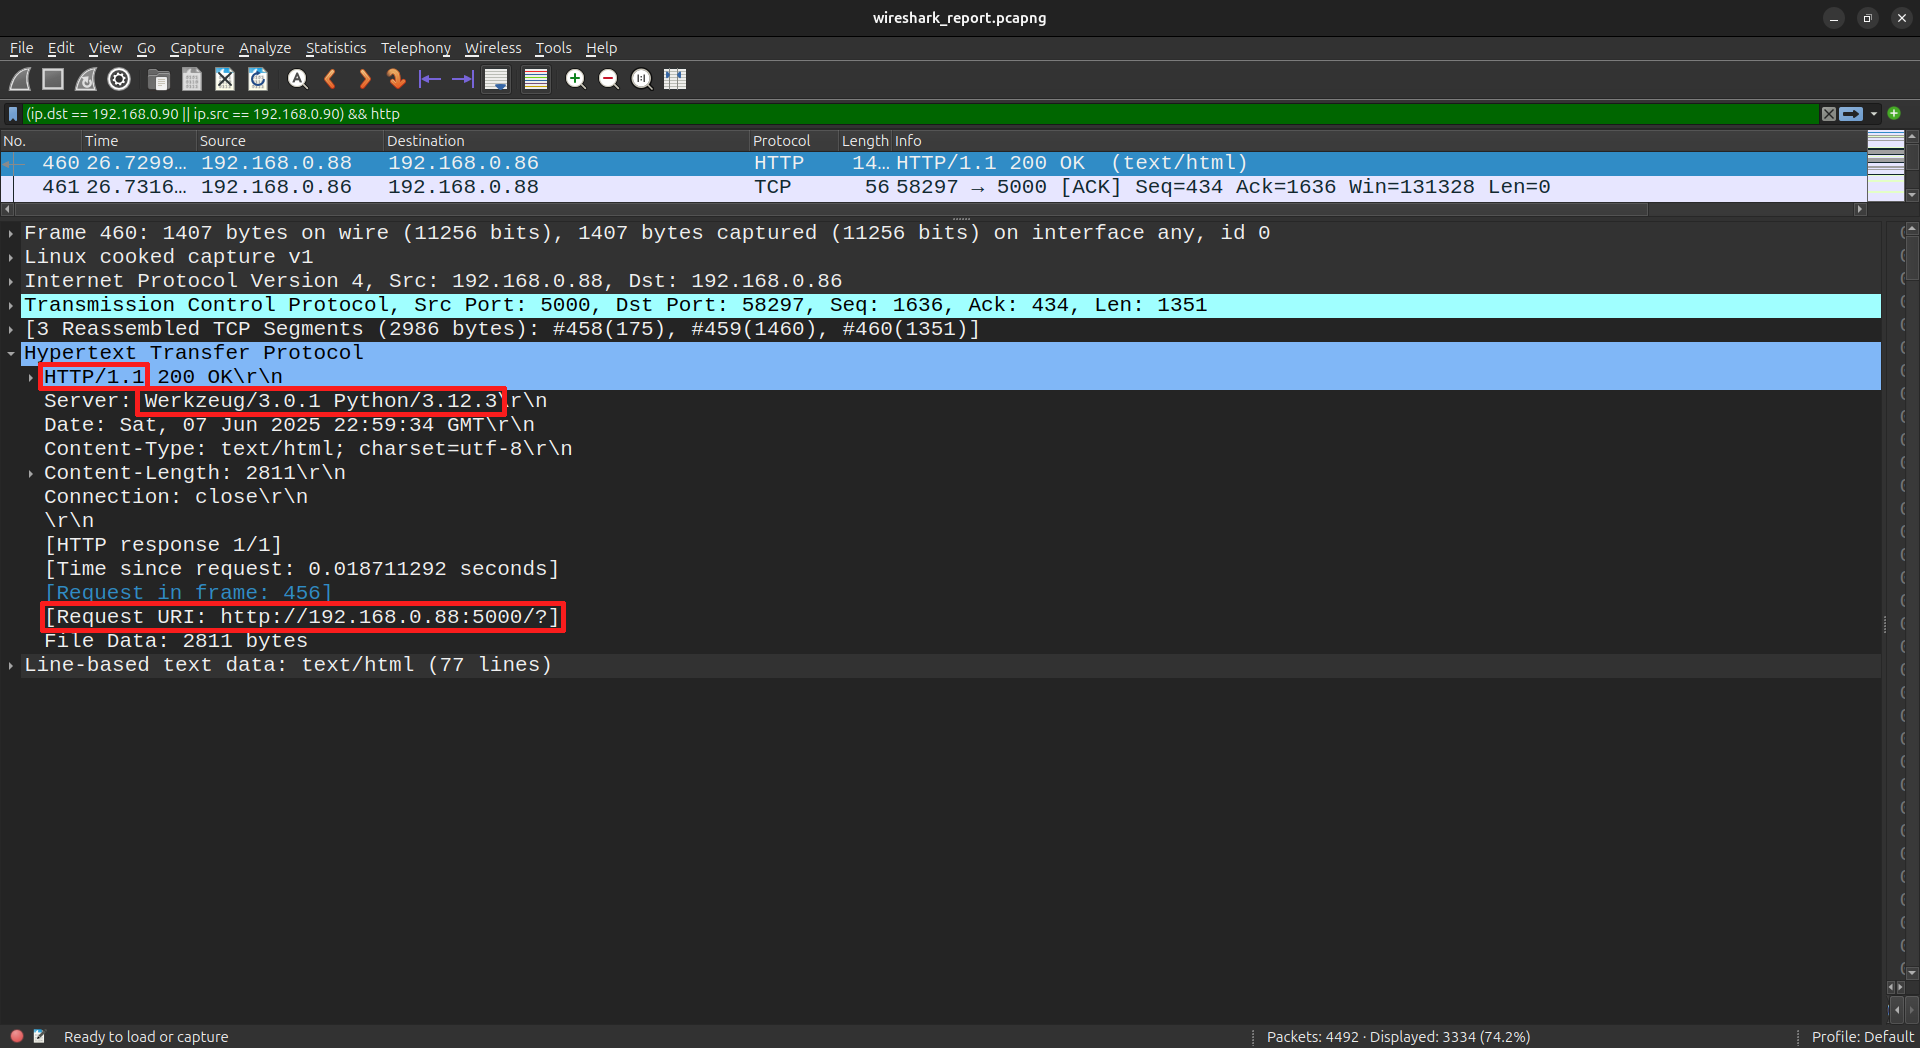
\includegraphics[width=\columnwidth]{../media/07-server_application.png}
\caption{Cabeçalho de aplicação da resposta à primeira requisição do Cliente 1}
\label{fig:application_header}
\end{figure}

\textbf{A.} Nas figuras 2 e 3, é possível notar as requisições HTTP do índice da página do serviço pelos Clientes 1 e 2, respectivamente. O primeiro opera em um Windows 10, com o navegador Chrome; e o segundo em um Android 10 baseado em Linux, também acessando o serviço pelo navegador Chrome (Mobile). Na figura 9, é visível que o servidor está operando na linguagem Python 3.12.3, representando uma aplicação Werkzeug na versão 3.0.1.

\textbf{B.} Nas figuras 2 e 3 estão representados os IPs dos clientes (192.168.0.86 e 192.168.0.71) e do servidor (192.168.0.88) operando na porta 5000.

\textbf{C.} Na figura 4, a resposta do servidor à requisição do arquivo tem uma carga útil de 1575 bytes, que coincide com o tamanho em bytes do arquivo no diretório local do servidor, como explícito na figura 5. Já na figura 6, o Cliente 1 envia uma mensagem gerada pelo SocketIO, pedindo o registro do cliente com o nome ``giovanni''. Isso demonstra que a troca de pacotes entre clientes e servidor e sua carga útil correspondem ao funcionamento esperado da aplicação desenvolvida.

\textbf{D.} Analisando os dados da resposta do servidor ao Cliente 1 que contém o índice da página HTML da aplicação, pode-se ver: na figura 7, os dados dos cabeçalhos das camadas de enlace e rede, que denotam, respectivamente, a tecnologia utilizada para transmissão (Ethernet), e uso do IPv4 no endereçamento de origem e destino do segmento encapsulado; na figura 8, o cabeçalho da camada de transporte, com as flags TCP (ACK, RST, SYN, FIN, etc.), dados da janela de transmissão, tamanho do cabeçalho e checksum da mensagem encapsulada; e, por fim, na figura 9, o cabeçalho HTTP/1.1, com o tamanho da mensagem enviada, o URI ao qual foi feita a requisição (com IP e porta) e o código da mensagem (200, OK), entre outras informações.


\section{Conclusão}

O desenvolvimento deste sistema de chat em tempo real proporcionou uma compreensão prática e aprofundada dos conceitos fundamentais de redes de computadores. A implementação bem-sucedida demonstra a viabilidade e eficiência das tecnologias WebSocket para aplicações que requerem comunicação bidirecional em tempo real.

\subsection{Principais Conquistas}

O desenvolvimento do ChatWeb 2.0 alcançou todos os objetivos estabelecidos, combinando funcionalidade técnica com uma experiência visual nostálgica autêntica:

\begin{itemize}
\item \textbf{Implementação Completa}: Sistema de chat multi-usuário totalmente funcional com criação dinâmica de salas
\item \textbf{Estética Nostálgica}: Interface que reproduz a experiência do Windows XP e início dos anos 2000
\item \textbf{Arquitetura Robusta}: Estrutura orientada a eventos com classes bem definidas e separação de responsabilidades
\item \textbf{Comunicação WebSocket}: Demonstração prática de protocolos modernos com análise detalhada de tráfego
\item \textbf{Validação e Robustez}: Sistema de validações que previne estados inconsistentes e trata erros adequadamente
\end{itemize}

\subsection{Aprendizados Técnicos}

O desenvolvimento do ChatWeb 2.0 proporcionou insights valiosos sobre programação de redes e desenvolvimento web moderno:

\textbf{Arquitetura Cliente-Servidor Moderna}: A implementação demonstrou como o paradigma orientado a eventos com WebSockets permite criar aplicações responsivas e escaláveis. O Flask-SocketIO abstraiu complexidades de baixo nível mantendo controle sobre o protocolo de comunicação.

\textbf{Gerenciamento de Estado Distribuído}: A sincronização entre múltiplos clientes revelou desafios únicos na manutenção de consistência. A abordagem de "fonte única da verdade" no servidor com propagação de eventos mostrou-se eficaz para manter todos os clientes sincronizados.

\textbf{Protocolos de Camada de Aplicação}: O Socket.IO demonstrou como protocolos de alto nível podem fornecer funcionalidades avançadas (como rooms, namespaces e reconnection) sobre WebSockets básicos, ilustrando a importância das abstrações de protocolo.

\textbf{Design de Interface}: A recriação da estética do Windows XP usando CSS moderno (flexbox, grid, box-shadow) demonstrou como técnicas contemporâneas podem replicar visuals clássicos, combinando o melhor de ambas as épocas.

\textbf{Modularização JavaScript}: A arquitetura em módulos ES6 permitiu separação clara de responsabilidades entre manipulação de DOM, comunicação de rede e lógica de apresentação, facilitando manutenção e evolução do código.

\textbf{Análise de Protocolos em Tempo Real}: O uso do Wireshark revelou detalhes fascinantes sobre como dados são transmitidos através das camadas de rede, desde frames Ethernet até mensagens Socket.IO, proporcionando visão prática da pilha TCP/IP.

\subsection{Limitações e Trabalhos Futuros}

Embora o ChatWeb 2.0 tenha alcançado seus objetivos educacionais, algumas limitações foram identificadas e representam oportunidades para evolução:

\textbf{Limitações Atuais}:
\begin{itemize}
\item \textbf{Persistência de Dados}: Mensagens e salas existem apenas durante a sessão do servidor
\item \textbf{Escalabilidade}: Armazenamento em memória limita o número de usuários e mensagens
\item \textbf{Autenticação}: Sistema atual usa apenas nomes de usuário sem senhas ou criptografia
\item \textbf{Suporte a Mídia}: Funcionalidade de arquivos e imagens foi parcialmente implementada
\item \textbf{Moderação}: Ausência de controles administrativos e filtros de conteúdo
\end{itemize}

\textbf{Oportunidades de Expansão}:
\begin{itemize}
\item \textbf{ChatWeb 3.0}: Evolução com banco de dados para persistência
\item \textbf{Recursos Nostálgicos}: Integração de emoticons pixelizados e sounds effects clássicos
\item \textbf{Salas Temáticas}: Implementação de temas visuais diferentes (Windows 98, Mac OS Classic, etc.)
\item \textbf{Bots e Easter Eggs}: Adição de elementos interativos que remetem à época
\item \textbf{Histórico de Conversas}: Sistema de logs e busca em mensagens antigas
\item \textbf{Status e Away Messages}: Funcionalidades características dos messengers clássicos
\end{itemize}

\textbf{Melhorias Técnicas}:
\begin{itemize}
\item Implementação de rate limiting para prevenir spam
\item Otimização de performance para milhares de usuários simultâneos
\item Adição de SSL/TLS para comunicação segura
\item Desenvolvimento de API REST complementar para integração
\item Implementação de testes automatizados unitários e de integração
\end{itemize}

\subsection{Considerações Finais}

O desenvolvimento do ChatWeb 2.0 representa uma síntese bem-sucedida entre aprendizado técnico e expressão criativa, demonstrando como projetos educacionais podem ir além da mera implementação funcional para criar experiências memoráveis e significativas.

\textbf{Impacto Educacional}: Este projeto demonstra como conceitos fundamentais de redes de computadores podem ser assimilados através de implementação prática. A combinação de programação client-server, análise de protocolos e design de interface proporcionou uma compreensão holística dos sistemas distribuídos modernos.

\textbf{Valor da Nostalgia Técnica}: A escolha estética do Windows XP não foi meramente decorativa, mas serviu como ponte entre tecnologias modernas (WebSockets, ES6, CSS3) e a experiência familiar de interfaces clássicas. Isso demonstra como o design pode facilitar a adoção e compreensão de tecnologias complexas.

\textbf{Validação Prática}: A análise detalhada do tráfego de rede com Wireshark confirmou o funcionamento correto de todos os protocolos envolvidos, desde frames Ethernet até mensagens Socket.IO. Essa validação empírica reforça a importância da experimentação prática no aprendizado de redes de computadores.

\textbf{Arquitetura para o Futuro}: A estrutura modular e orientada a eventos criada no ChatWeb 2.0 estabelece uma base sólida para evoluções futuras, seja na direção de maior escala, funcionalidades avançadas ou diferentes temáticas nostálgicas.

O sucesso deste projeto evidencia que o aprendizado de redes de computadores pode ser simultaneamente rigoroso e divertido, técnico e criativo, moderno e nostálgico. O ChatWeb 2.0 não apenas cumpriu seus objetivos educacionais, mas criou uma experiência única que celebra tanto a evolução tecnológica quanto a nostalgia pelos primórdios da internet.

% trigger a \newpage just before the given reference
% number - used to balance the columns on the last page
% adjust value as needed - may need to be readjusted if
% the document is modified later
%\IEEEtriggeratref{8}
% The "triggered" command can be changed if desired:
%\IEEEtriggercmd{\enlargethispage{-5in}}

% references section

% can use a bibliography generated by BibTeX as a .bbl file
% BibTeX documentation can be easily obtained at:
% http://mirror.ctan.org/biblio/bibtex/contrib/doc/
% The IEEEtran BibTeX style support page is at:
% http://www.michaelshell.org/tex/ieeetran/bibtex/
%\bibliographystyle{IEEEtran}
% argument is your BibTeX string definitions and bibliography database(s)
%\bibliography{IEEEabrv,../bib/paper}
%
% <OR> manually copy in the resultant .bbl file
% set second argument of \begin to the number of references
% (used to reserve space for the reference number labels box)
\begin{thebibliography}{9}

\bibitem{rfc6455}
I.~Fette and A.~Melnikov, ``The WebSocket Protocol,'' RFC 6455, 
Internet Engineering Task Force, December 2011. [Online]. Available: 
https://tools.ietf.org/html/rfc6455

\bibitem{socketio}
Socket.IO Development Team, ``Socket.IO - Realtime application framework,'' 
[Online]. Available: https://socket.io/

\bibitem{flask}
A.~Ronacher, ``Flask - A Python Microframework,'' 
[Online]. Available: https://flask.palletsprojects.com/

\bibitem{flasksocketio}
M.~Grinberg, ``Flask-SocketIO - Socket.IO integration for Flask applications,'' 
[Online]. Available: https://flask-socketio.readthedocs.io/

\bibitem{wireshark}
Wireshark Foundation, ``Wireshark - Network Protocol Analyzer,'' 
[Online]. Available: https://www.wireshark.org/

\bibitem{tcp}
J.~Postel, ``Transmission Control Protocol,'' RFC 793, 
Internet Engineering Task Force, September 1981. [Online]. Available: 
https://tools.ietf.org/html/rfc793

\bibitem{http11}
R.~Fielding et al., ``Hypertext Transfer Protocol -- HTTP/1.1,'' RFC 2616, 
Internet Engineering Task Force, June 1999. [Online]. Available: 
https://tools.ietf.org/html/rfc2616

\bibitem{realtime}
L.~Richardson and S.~Ruby, \emph{RESTful Web Services}, 1st~ed.\hskip 1em plus
  0.5em minus 0.4em\relax O'Reilly Media, 2007.

\bibitem{websocket_book}
A.~Lombardi, \emph{WebSocket - Lightweight Client-Server Communications}, 1st~ed.\hskip 1em plus
  0.5em minus 0.4em\relax O'Reilly Media, 2015.

\bibitem{kurose}
J.~F.~Kurose and K.~W.~Ross, \emph{Computer Networking: A Top-Down Approach}, 8th~ed.\hskip 1em plus
  0.5em minus 0.4em\relax Pearson, 2021.

\bibitem{gabrielcarvfer}
G.~Carvalho, ``Redes-de-Computadores-UnB - Material de apoio para disciplina de Redes de Computadores,'' 
[Online]. Available: https://github.com/Gabrielcarvfer/Redes-de-Computadores-UnB

\bibitem{mdn}
Mozilla Developer Network, ``Web technology for developers,'' 
[Online]. Available: https://developer.mozilla.org/en-US/docs/Web

\end{thebibliography}
\end{otherlanguage}

\end{document}